\documentclass[sigconf,anonymous,review]{acmart}

\acmConference{CIKM '26}{November 7--11, 2026}{Rome, Italy}
\acmYear{2026}
\copyrightyear{2026}

\usepackage{booktabs}
\usepackage{algorithm}
\usepackage{algpseudocode}
\usepackage{amsmath}
\usepackage{amssymb}
\usepackage{graphicx}
\usepackage{pgfplots}
\pgfplotsset{compat=1.18}
\usepackage{tikz}
\usetikzlibrary{shapes.geometric, arrows.meta, positioning, fit, backgrounds}
\usepackage{subcaption}
\usepackage{multirow}
\usepackage{xspace}
\usepackage{microtype}
\usepackage{listings}
\lstset{basicstyle=\ttfamily\scriptsize, breaklines=true, frame=none,
        aboveskip=2pt, belowskip=2pt}

\settopmatter{printfolios=true}
\setcopyright{none}
\renewcommand\footnotetextcopyrightpermission[1]{}
\setlength{\textfloatsep}{5pt plus 1pt minus 1pt}
\setlength{\floatsep}{5pt plus 1pt minus 1pt}
\setlength{\intextsep}{5pt plus 1pt minus 1pt}
\setlength{\abovecaptionskip}{3pt}
\setlength{\belowcaptionskip}{2pt}
\setlength{\tabcolsep}{3pt}

\newcommand{\votr}{\textsc{VOTR}\xspace}
\newcommand{\mcpzero}{MCP-Zero\xspace}
\newcommand{\topk}{Top-$k$\xspace}
\newcommand{\hdatk}{Hd@$k$\xspace}

\title{VOTR: Vector Orchestrated Tool Retrieval for Scalable Multi-Agent Systems}

\begin{document}

\begin{abstract}
Large language model agents using the Model Context Protocol (MCP) face prohibitive
token costs when injecting full tool catalogues into every request.
\mcpzero established embedding-based retrieval as viable but remains a research
prototype with a static index, fixed top-$k$, and no production deployment
capabilities.
\votr introduces a hybrid retrieval pipeline that fuses dense embeddings, BM25,
and SPLADE-lite with weighted Reciprocal Rank Fusion and field-aware re-ranking
over structured MCP metadata.
It adds calibrated adaptive candidate selection through a score-gap policy that
expands the candidate set only when retrieval confidence is low.
It also provides production infrastructure for zero-downtime server registration,
overlap-aware disambiguation, abstention guarding, and compressed schema injection.
On a 500-query benchmark spanning 309 MCP servers and 2,806 tools, \votr achieves
96.8\% Top-1 accuracy [95\% CI: 95.0, 98.2] at sub-350ms median latency with an
average context injection of 230 tokens---a 99.91\% reduction relative to
full-catalogue injection.
On single-hop routing, \votr achieves 96.8\% Top-1 accuracy; on 5-step compound
chains, it achieves 87\% chain success at $k=1$ (96\% at $k=5$), with a 100\%
abstention pass rate on adversarial negative-control queries.
Multi-hop chains over 50 unique servers achieve 100\% hop-level and chain success.
\votr is the first MCP tool retrieval service combining hybrid retrieval, a dynamic
registry, and safety mechanisms in a production-deployable architecture.
\end{abstract}

\begin{CCSXML}
<ccs2012>
  <concept>
    <concept_id>10002951.10003317.10003347.10003350</concept_id>
    <concept_desc>Information systems~Query reformulation</concept_desc>
    <concept_significance>500</concept_significance>
  </concept>
  <concept>
    <concept_id>10002951.10003317.10003325.10003326</concept_id>
    <concept_desc>Information systems~Retrieval models and ranking</concept_desc>
    <concept_significance>500</concept_significance>
  </concept>
  <concept>
    <concept_id>10010147.10010178.10010224</concept_id>
    <concept_desc>Computing methodologies~Autonomous agents</concept_desc>
    <concept_significance>300</concept_significance>
  </concept>
</ccs2012>
\end{CCSXML}
\ccsdesc[500]{Information systems~Retrieval models and ranking}
\ccsdesc[300]{Computing methodologies~Autonomous agents}
\keywords{Model Context Protocol, tool retrieval, hybrid retrieval,
          LLM agents, agentic AI, multi-agent systems}

\maketitle

%% ============================================================
\section{Introduction}
%% ============================================================

By early 2025, over 3,000 community-built MCP servers had been published.
Injecting the full tool catalogue from a deployment of 309 servers and 2,806 tools
into an LLM context consumes approximately 262,000 tokens per query---tokens
unavailable for reasoning about the user's actual request.
MCP standardises tool access through a transport-agnostic JSON-RPC interface, but
this standardisation shifts the systems bottleneck from tool wiring to tool
selection at catalogue scale~\cite{anthropic_mcp2024,mcpzero2025}.

Beyond token efficiency, tool retrieval is a foundational capability for reliable
agentic systems.
An agent that selects the wrong tool---or injects too many tools and confuses the
LLM's reasoning---fails at the task level regardless of the quality of its planning.
\votr addresses tool retrieval as a first-class infrastructure problem: accurate
enough for automated multi-hop chains (87\% 5-step success, 100\% on 50-hop unique
server chains), safe enough to abstain when no tool matches (100\% adversarial pass
rate), and fast enough for interactive agent loops (sub-350ms).
These properties together make \votr an enabling layer for production multi-agent
systems, not merely a token optimisation.

Naive retrieval is insufficient because MCP tool routing is not ordinary document
retrieval.
Tool names are identifier-heavy, descriptions are shallow and variable in quality,
multiple servers expose overlapping capabilities, and each surplus candidate carries
a hard context-budget cost.
These four properties make exact lexical matching, semantic matching, overlap
detection, and adaptive candidate sizing jointly necessary---no single retrieval
signal addresses all of them (Section~\ref{sec:background}).

\mcpzero demonstrated that proactive retrieval can achieve 95.2\% Top-1 accuracy
and approximately 98\% token reduction~\cite{mcpzero2025}.
However, it leaves four production gaps: a static index, no live transport
discovery, fixed top-$k$ selection, and no safety mechanisms for ambiguity or
unsupported intents.
\votr addresses these gaps as a production retrieval layer for MCP deployments.

\votr routes each request through a hybrid retrieval stack, calibrates the number
of candidates handed to the downstream LLM, and supports live registry updates
without restarting the service.
On the full 309-server, 2,806-tool catalogue, it achieves 96.8\% Top-1 accuracy,
sub-350ms median latency, 230 tokens average injection, and 99.91\% token reduction
relative to full-catalogue injection.

This paper makes three contributions:
\begin{itemize}
\item \textbf{C1---Hybrid Retrieval Pipeline:} A production retrieval system fusing
  dense embeddings, BM25, and SPLADE-lite via weighted Reciprocal Rank Fusion, with
  field-aware re-ranking over structured tool metadata.
\item \textbf{C2---Calibrated Adaptive Candidate Selection:} A score-gap calibration
  mechanism inspired by conformal prediction non-conformity scoring that dynamically
  selects the number of tool candidates based on retrieval confidence, reducing
  average context injection while maintaining coverage.
\item \textbf{C3---Production Deployment Infrastructure:} Zero-downtime hot server
  registration, overlap-aware disambiguation, abstention guarding, and compressed
  schema injection enabling real-world MCP deployment.
\end{itemize}

%% ============================================================
\section{Background and Related Work}
\label{sec:background}
%% ============================================================

\subsection{The Model Context Protocol}
MCP is an open standard for connecting AI assistants to tools and data sources
through a JSON-RPC interface~\cite{anthropic_mcp2024}.
Servers expose capabilities through endpoints such as \texttt{tools/list} and can
be reached over stdio or HTTP/SSE transports.
This decoupling amplifies the retrieval challenge as the catalogue grows.

\subsection{Tool Retrieval for LLM Agents}
ToolBench and ToolLLM study large-scale API use and tool-learning benchmarks for
LLMs~\cite{toolbench2024}.
ToolkenGPT represents tools as learned embeddings for frozen language
models~\cite{toolkengpt2023}.
Retrieval-augmented generation (RAG) motivates retrieving external context instead
of placing all context in the prompt~\cite{lewis2020rag}.
\mcpzero adapts this idea to MCP tool retrieval~\cite{mcpzero2025}.
RAG-MCP studies retrieval to mitigate prompt bloat in MCP tool
selection~\cite{rag_mcp_2025}.
Dynamic ReAct explores scalable tool selection for large MCP
environments~\cite{dynamic_react_2025}.
Tool-to-Agent Retrieval identifies the need to retrieve across coupled tool-agent
structures~\cite{tool_to_agent_2025}.
\votr addresses the production deployment gap left by \mcpzero and the
intent-decomposition gap identified by Tool-to-Agent Retrieval.

\subsection{Sparse, Dense, and Hybrid Retrieval}
BM25 remains a strong lexical ranking baseline~\cite{robertson2009bm25}, while
DPR-style dense retrieval improves semantic matching under
paraphrase~\cite{karpukhin2020dpr}.
SPLADE learns sparse lexical expansion from language-model
activations~\cite{formal2021splade}, and RRF provides a robust rank-level method
for combining heterogeneous retrieval lists~\cite{cormack2009rrf}.

MCP tool retrieval exhibits four properties that make standard retrieval methods
individually insufficient.
\textbf{(i)~Identifier-heavy vocabulary:} Tool names are camelCase or snake\_case
identifiers (e.g., \texttt{search\_repositories}).
Embedding models trained on prose fragment these inconsistently, while BM25 with
identifier normalisation handles them precisely.
\textbf{(ii)~Variable description quality:} Community MCP manifests range from
one-sentence stubs to full documentation.
Dense retrieval quality degrades with short or generic descriptions; BM25's
term-frequency weighting is more robust to this variance.
\textbf{(iii)~Cross-server capability overlap:} Multiple servers expose functionally
identical tools (e.g., code-hosting servers expose \texttt{search\_repositories}).
Standard IR treats documents as distinct; MCP routing requires explicit overlap
detection.
\textbf{(iv)~Hard context budget consequences:} Unlike document retrieval where
surplus candidates carry low cost, each surplus tool schema consumes roughly 93
tokens and can degrade LLM reasoning quality~\cite{mcpzero2025}.
This makes adaptive candidate sizing a first-class requirement, not an optimisation.

\subsection{Calibrated Uncertainty in Retrieval}
Conformal prediction~\cite{shafer2008tutorial} provides distribution-free coverage
guarantees via non-conformity scoring.
We draw on this framework conceptually to motivate our score-gap calibration
mechanism; however, our deployed policy combines engineered retrieval features with
heuristic structural signals and does not claim formal conformal coverage
guarantees---it functions as a calibrated empirical handoff policy.
Q-RAG similarly studies retrieval-time value estimation for multi-step long-context
retrieval~\cite{qrag2026}.

%% ============================================================
\section{The VOTR System}
%% ============================================================

\subsection{Architectural Overview}

\begin{figure*}[t]
\centering
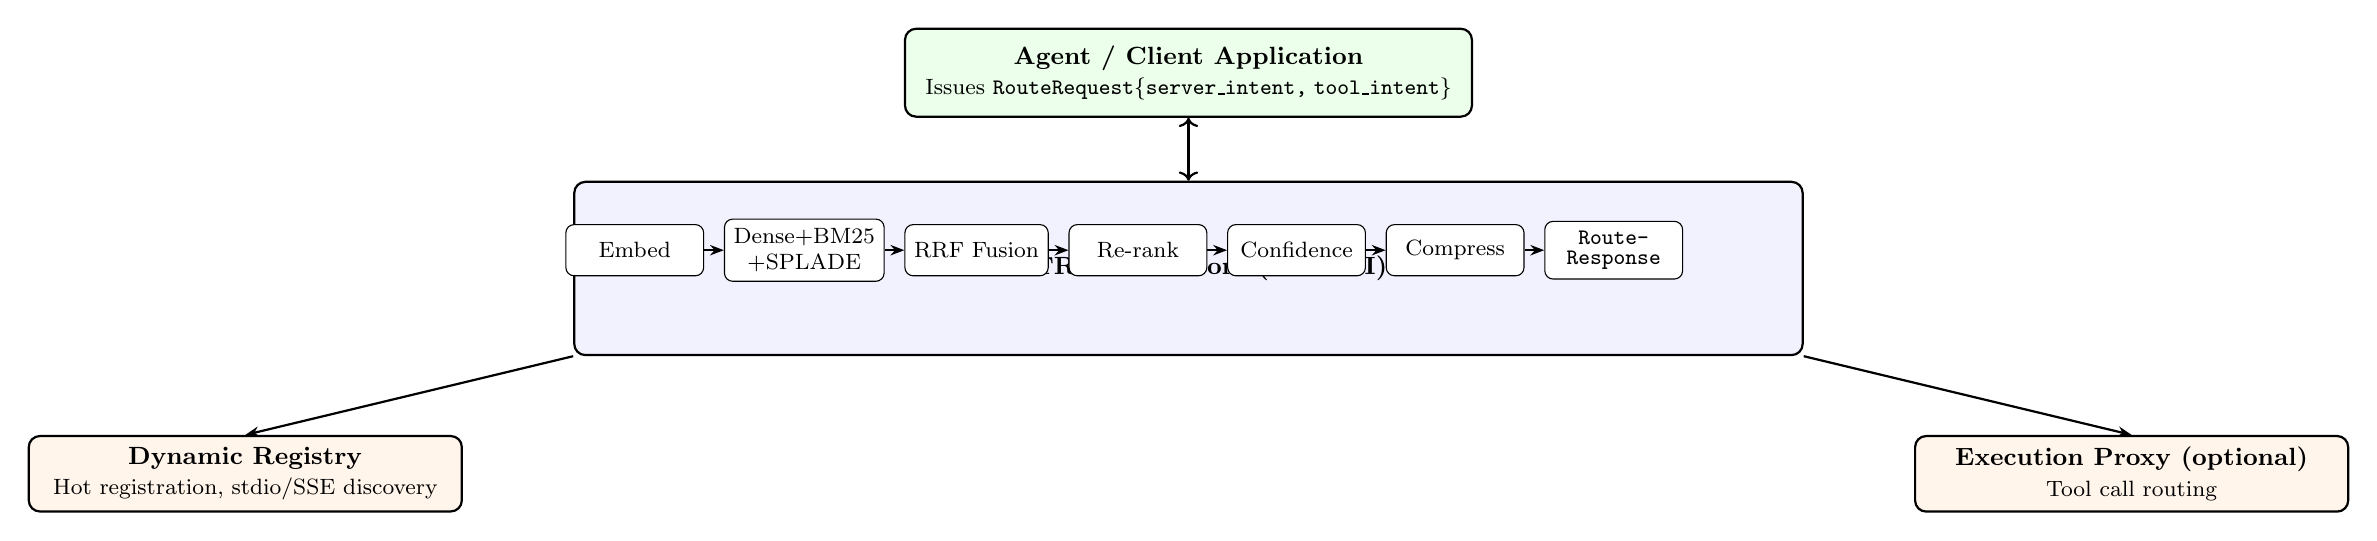
\begin{tikzpicture}[
  font=\small,
  box/.style={draw, rounded corners=4pt, align=center, fill=blue!5,
              thick, inner sep=6pt},
  smallbox/.style={draw, rounded corners=4pt, align=center, fill=orange!8,
                   thick, inner sep=4pt},
  stage/.style={draw, rounded corners=3pt, align=center, fill=white,
                minimum width=1.75cm, minimum height=0.65cm, font=\footnotesize},
  arr/.style={-{Stealth[length=5pt]}, thick},
  node distance=0.45cm
]
\node[box, fill=green!8, minimum width=7.2cm] (agent)
  {\textbf{Agent / Client Application}\\
   {\footnotesize Issues \texttt{RouteRequest\{server\_intent,\;tool\_intent\}}}};
\node[box, below=0.8cm of agent, minimum width=15.6cm, minimum height=2.2cm]
  (router) {\textbf{VOTR Router Core (FastAPI)}};
\node[stage, below left=0.55cm and 6.15cm of router.north] (embed)  {Embed};
\node[stage, right=0.25cm of embed]   (retrieve) {Dense+BM25\\+SPLADE};
\node[stage, right=0.25cm of retrieve](fusion)   {RRF Fusion};
\node[stage, right=0.25cm of fusion]  (rerank)   {Re-rank};
\node[stage, right=0.25cm of rerank]  (conf)     {Confidence};
\node[stage, right=0.25cm of conf]    (compress)  {Compress};
\node[stage, right=0.25cm of compress](resp)
  {\texttt{Route-}\\[-2pt]\texttt{Response}};
\draw[arr] (embed)--(retrieve); \draw[arr] (retrieve)--(fusion);
\draw[arr] (fusion)--(rerank);  \draw[arr] (rerank)--(conf);
\draw[arr] (conf)--(compress);  \draw[arr] (compress)--(resp);
\node[smallbox, below left=1.0cm and 1.4cm of router, minimum width=5.5cm]
  (reg)   {\textbf{Dynamic Registry}\\{\footnotesize Hot registration, stdio/SSE discovery}};
\node[smallbox, below right=1.0cm and 1.4cm of router, minimum width=5.5cm]
  (proxy) {\textbf{Execution Proxy (optional)}\\{\footnotesize Tool call routing}};
\draw[arr, <->] (agent)--(router);
\draw[arr] (router.south west)--(reg.north);
\draw[arr] (router.south east)--(proxy.north);
\end{tikzpicture}
\caption{VOTR three-tier architecture. The Router Core orchestrates the full
retrieval pipeline per request. The Registry enables zero-downtime server
registration without restarting the service.}
\label{fig:arch}
\end{figure*}

\votr is structured as a three-tier service (Figure~\ref{fig:arch}).
The top tier is the agent or client application, which submits a routing request
containing separate natural-language server and tool intents.
The middle tier is the Router Core, a FastAPI service that embeds the request,
retrieves candidates, fuses rankings, re-ranks structured fields, estimates
confidence, compresses schemas, and returns a \texttt{RouteResponse}.
The bottom tier contains the Dynamic Registry and optional Execution Proxy.

The Vector Store uses \texttt{meta.json} for server/tool metadata and \texttt{.npy}
shards for dense arrays, enabling incremental updates unlike \mcpzero's single
326\,MB JSON file (Table~\ref{tab:index}).

\begin{table}[t]
\centering
\small
\caption{Index format comparison. VOTR's sharded binary format enables incremental
hot registration without full rebuilds.}
\label{tab:index}
\begin{tabular}{@{}lll@{}}
\toprule
Aspect & \mcpzero & \votr \\
\midrule
Storage format    & Single 326\,MB JSON & \texttt{meta.json} + \texttt{.npy} shards \\
Rebuild strategy  & Full manual rebuild & Incremental hot registration \\
Embedding storage & Inline in JSON      & Separate binary arrays \\
Memory footprint  & Entire file in RAM  & Memory-mapped arrays \\
Parse method      & Full JSON load      & Streaming build path \\
\bottomrule
\end{tabular}
\end{table}

\subsection{Request Lifecycle}
A \texttt{/route} call proceeds as follows:
(1)~embed \texttt{server\_intent} and \texttt{tool\_intent} via the OpenAI API into
two 3072-dimensional vectors;
(2)~hierarchical dense server scoring to obtain a top-$N$ server pool;
(3)~BM25 and SPLADE-lite scoring over all tool documents in parallel;
(4)~weighted RRF fusion;
(5)~field-aware re-ranking of the top-$H$ candidates;
(6)~non-conformity score, confidence tier, and adaptive-$k$;
(7)~overlap detection and abstention guard; and
(8)~schema compression into the returned \texttt{RouteResponse}.
Embedding dominates latency at approximately 200--280\,ms via the OpenAI API;
local retrieval and re-ranking add under 20\,ms.
The service exposes \texttt{/route}, \texttt{/register}, and
\texttt{/register/discover} (stdio) / \texttt{/register/discover/sse} (HTTP/SSE).

\textbf{Schema compression.}
\mcpzero-style injection serialises full JSON schemas ($\sim$93 tokens/tool).
\votr compresses each tool to a single structured line:
\begin{lstlisting}
[git-hosting] search_repositories(query:str, page?:int)
  -> Search repositories matching a query.
\end{lstlisting}
This reduces mean tokens per tool from 93.5 to 26.2 (72\% reduction), compounding
with adaptive-$k$ to yield 230 tokens average end-to-end injection.

%% ============================================================
\section{Retrieval Pipeline}
%% ============================================================

\subsection{Hierarchical Dense Retrieval}
Given server intent embedding $\mathbf{q}_s$ and tool intent embedding
$\mathbf{q}_t$, \votr scores server $i$ using Equation~\eqref{eq:server_score}:
\begin{equation}
\label{eq:server_score}
  \sigma_i =
  \frac{
    w_{\max}\max\!\bigl(\cos(\mathbf{q}_s,\mathbf{e}^{(i)}_{\mathrm{desc}}),
                        \cos(\mathbf{q}_s,\mathbf{e}^{(i)}_{\mathrm{sum}})\bigr)
    + w_{\mathrm{mean}}\dfrac{\cos(\mathbf{q}_s,\mathbf{e}^{(i)}_{\mathrm{desc}})
                 + \cos(\mathbf{q}_s,\mathbf{e}^{(i)}_{\mathrm{sum}})}{2}
  }{w_{\max}+w_{\mathrm{mean}}}.
\end{equation}
The default uses $w_{\max}=1.0$, $w_{\mathrm{mean}}=0.0$, top-$N=8$ servers.
For tool $j$ in the resulting pool, Equation~\eqref{eq:tool_score} defines the
dense score:
\begin{equation}
\label{eq:tool_score}
  \tau_j = \sigma_{\pi(j)} \cdot t_j \cdot \max(\sigma_{\pi(j)},\, t_j),
  \qquad
  t_j = \cos(\mathbf{q}_t,\mathbf{e}^{\mathrm{tool}}_j),
\end{equation}
where $\pi(j)$ maps a tool to its parent server.
This multiplicative formulation requires alignment on both server and tool
dimensions, directly addressing cross-server capability overlap.

\subsection{BM25 Sparse Retrieval}
Each tool is represented as the BM25 document in Equation~\eqref{eq:doc_concat}:
\begin{equation}
\label{eq:doc_concat}
  d_j = s_{\mathrm{name}}^{(\pi(j))} \Vert s_{\mathrm{sum}}^{(\pi(j))}
        \Vert s_{\mathrm{desc}}^{(\pi(j))} \Vert
        t_{\mathrm{name}}^{(j)} \Vert t_{\mathrm{desc}}^{(j)}.
\end{equation}
Normalisation splits camelCase and snake\_case, normalises separators, strips light
plurals, and intentionally avoids deduplication so BM25 term-frequency signals
remain available.

\subsection{SPLADE-lite Lexical Expansion}
Full SPLADE requires GPU inference~\cite{formal2021splade}.
\votr instead uses TF-IDF with unigram and bigram features, sublinear TF scaling,
and L2 normalisation, approximating SPLADE's compound-term sensitivity through
bigram features (e.g., ``search repositories'') at negligible inference cost.
Fusion weight: $w_{\mathrm{splade}}=0.50$.

\subsection{Reciprocal Rank Fusion}
The three ranked lists are combined by weighted RRF (Equation~\eqref{eq:rrf}):
\begin{equation}
\label{eq:rrf}
  \mathrm{RRF}(j)=\sum_{\ell=1}^{3}\frac{w_\ell}{k+r_\ell(j)},
\end{equation}
with $k=60$, $w_{\mathrm{dense}}=1.0$, $w_{\mathrm{BM25}}=1.0$,
$w_{\mathrm{SPLADE}}=0.50$~\cite{cormack2009rrf}.
Algorithm~\ref{alg:rrf} gives the weighted implementation.

\begin{algorithm}[t]
\caption{Weighted Reciprocal Rank Fusion}
\label{alg:rrf}
\begin{algorithmic}[1]
\Require Lists $\mathcal{L}_1,\ldots,\mathcal{L}_L$, weights $w_1,\ldots,w_L$, $k$
\Ensure Score map $S$
\State $S \gets \emptyset$
\For{$\ell = 1$ \textbf{to} $L$}
  \For{$r = 1$ \textbf{to} $|\mathcal{L}_\ell|$}
    \State $S[\mathcal{L}_\ell[r]] \mathrel{+}= w_\ell/(k+r)$
  \EndFor
\EndFor
\State \Return $S$
\end{algorithmic}
\end{algorithm}

\subsection{Field-Aware Re-ranking}
The top-$H$ fused candidates receive the field bonus in
Equation~\eqref{eq:field_bonus}:
\begin{equation}
\label{eq:field_bonus}
  B_j = \sum_{f\in\mathcal{F}} w_f \cdot
  \mathrm{Dice}(Q_f,T_j^f) + w_{\mathrm{expl}}\mathbf{1}[\hat{s}=s_j],
\end{equation}
where Dice is the token-level S{\o}rensen--Dice coefficient.
Equation~\eqref{eq:adj_score} gives the final adjusted score:
\begin{equation}
\label{eq:adj_score}
  \hat{\tau}_j = \mathrm{RRF}(j) + \lambda B_j
  + \mu\max\!\bigl(0,\cos(\mathbf{q}_t,\mathbf{e}^{\mathrm{tool}}_j)\bigr).
\end{equation}

\begin{table}[t]
\centering
\caption{Field-aware re-ranking weights. Tool name receives highest weight as exact
function-name matches are the strongest relevance signal in MCP routing.}
\label{tab:field_weights}
\begin{tabular}{@{}lr@{}}
\toprule
Field & Weight \\
\midrule
Tool name             & 0.35 \\
Server name           & 0.25 \\
Tool description      & 0.20 \\
Parameters            & 0.12 \\
Server summary        & 0.08 \\
Explicit server boost & 0.22 \\
\bottomrule
\end{tabular}
\end{table}

A lightweight intent classifier penalises bulk-operation tools by factor 0.82 when
singular destructive intent is detected, and boosts them by factor 1.08 for
explicit batch intents.

%% ============================================================
\section{Confidence-Gated Handoff}
%% ============================================================

\subsection{Adaptive Top-\texorpdfstring{$K$}{K} Selection}
Algorithm~\ref{alg:adaptivek} uses three branches: gap $\ge \delta_c$ returns
$k_{\min}=1$; gap $\ge 0.5\delta_c$ returns 3; otherwise $k_{\max}$.
Default: $\delta_c=0.12$.

\begin{algorithm}[t]
\caption{Adaptive Top-$K$ Selection}
\label{alg:adaptivek}
\begin{algorithmic}[1]
\Require Scores $s_1\ge\cdots\ge s_n$, threshold $\delta_c$, bounds $k_{\min},k_{\max}$
\If{$n\le1$} \State \Return $\min(n,k_{\min})$ \EndIf
\State $\mathrm{gap}\gets s_1-s_2$
\If{$\mathrm{gap}\ge\delta_c$} \State \Return $k_{\min}$
\ElsIf{$\mathrm{gap}\ge 0.5\delta_c$} \State \Return $\min(3,n,k_{\max})$
\Else \State \Return $\min(k_{\max},n)$
\EndIf
\end{algorithmic}
\end{algorithm}

\subsection{Calibrated Score-Gap Policy}
Inspired by the non-conformity scoring concept in conformal
prediction~\cite{shafer2008tutorial}, but without claiming distribution-free
coverage guarantees (see Section~\ref{sec:background}), we define:
\begin{align}
\mathrm{nc}(q) &=
  \underbrace{-\log_{10}(\max(\delta,10^{-9}))-3}_{f(\delta)\ \text{gap signal}}
  \notag \\
  &+\underbrace{0.5\!\left(\tfrac{s_2}{s_1}-0.975\right)}_{g(s_1,s_2)\ \text{ratio signal}}
  -\underbrace{0.3\,\mathbf{1}[\hat{s}=s_{j^*}]}_{h(\hat{s})\ \text{server match bonus}}.
\label{eq:nc_score}
\end{align}
Lower scores indicate greater retrieval confidence.

\begin{table}[t]
\centering
\small
\caption{Confidence-based handoff tiers.}
\label{tab:tiers}
\begin{tabular}{@{}llll@{}}
\toprule
Tier   & nc Condition                    & Handoff-$k$ & Rationale \\
\midrule
High   & $\mathrm{nc}\le\tau_1$          & 1           & Clear top tool \\
Medium & $\tau_1<\mathrm{nc}\le\tau_3$   & 3           & Near-tie set \\
Low    & $\mathrm{nc}>\tau_3$            & 5           & Ambiguous query \\
\bottomrule
\end{tabular}
\end{table}

\subsection{Calibration}
Calibration uses \texttt{single\_tool.clean.json} ($n=500$), deterministic 80/20
split ($n=400$ calibration, $n=100$ validation).
From \texttt{conformal\_calibration.json}: $\tau_1=-0.242075$,
$\tau_3=-0.088911$, $\tau_{\mathrm{null}}=0.211089$.
Note: $\tau_{\mathrm{null}}$ is an nc-score threshold; it is distinct from the
query-support abstention threshold $\theta_{\mathrm{null}}=0.213$ in
Section~\ref{sec:robustness}, which operates on a different signal.
Runtime headline results use the gap-threshold policy
(\texttt{conformal\_enabled=false}).

%% ============================================================
\section{Robustness and Dynamic Registry}
\label{sec:robustness}
%% ============================================================

\subsection{Safety Mechanisms}
The abstention guard is two-stage.
First, if normalised query support $<\theta_q=0.18$ and server support
$<\theta_s=0.12$, confidence is downgraded to low and handoff-$k$ is floored at 5.
Second, if query support $<\theta_{\mathrm{null}}=0.213$, tool support $\le0.4$,
and no explicit server is named, \votr returns an empty candidate list, preventing
the LLM from fabricating tool calls against low-quality matches.

Overlap-aware disambiguation builds capability signatures from normalised name and
parameter tokens.
When the top tool belongs to a cluster within score window $\delta_{\mathrm{ov}}=0.0025$,
\votr sets \texttt{overlap\_ambiguous=true}, expands handoff-$k$, and downgrades
the confidence tier.
The regression suite (16 adversarial queries) achieves 100\% pass rate.

\subsection{Zero-Downtime Hot Registration}
New servers are registered by: (1)~validating name uniqueness, (2)~embedding server
description, server summary, and all tool descriptions via the embedding API,
(3)~extending the NumPy index arrays, (4)~rebuilding BM25 and SPLADE-lite indices,
and (5)~atomically swapping the engine's live index reference under CPython's GIL.
In-flight requests using the pre-swap index complete normally.

%% ============================================================
\section{Evaluation}
%% ============================================================

\subsection{Experimental Setup}
The evaluation catalogue contains 309 servers and 2,806 tools.
Embeddings use OpenAI \texttt{text-embedding-3-large} (3072 dimensions) as the
primary backbone; Section~\ref{sec:backbone} reports results for four additional
backbones.
The service runs as a FastAPI single-process deployment in the
\texttt{full\_stack} configuration.

All functional-correctness results measure closed-catalogue routing
accuracy---the ability to identify the correct tool among indexed servers using
queries derived from the same catalogue.
They do not measure generalisation to unseen server descriptions or
out-of-vocabulary tool names.
LiveMCPBench (Section~\ref{sec:external}) provides the primary out-of-distribution
evaluation signal, as its task traces are constructed independently of our
index~\cite{livemcpbench2025}.

RAG-MCP~\cite{rag_mcp_2025} and Dynamic ReAct~\cite{dynamic_react_2025} are
concurrent systems addressing related problems but do not provide public
implementations compatible with our benchmark protocol.
Tool-to-Agent Retrieval~\cite{tool_to_agent_2025} is evaluated on LiveMCPBench
under a shared protocol in Section~\ref{sec:external}.
Direct comparison against additional baselines on our closed-catalogue benchmark
remains future work.

\subsection{Main Results}

\begin{table*}[t]
\centering
\small
\caption{Full-stack functional correctness (primary evaluation,
\texttt{single\_tool.clean.report.json}). Low-cardinality one-server deployments
achieve ceiling-level accuracy. On the full 309-server catalogue, \votr improves
over the \mcpzero baseline~\cite{mcpzero2025} while adding production deployment
capabilities. Chn@$k$ = Chain Success requiring all steps correct.
``--'' indicates not reported in the cited work.}
\label{tab:main}
\begin{tabular}{@{}llccccccc@{}}
\toprule
Task & Scale & T1 & T3 & T5 & Hd@$k$ & Chn@1 & Chn@5 & Eq.T1 \\
\midrule
single\_tool & Finance (100)     & 1.000 & 1.000 & 1.000 & 1.000 & --    & --    & 1.000 \\
single\_tool & GitHub (100)      & 1.000 & 1.000 & 1.000 & 1.000 & --    & --    & 1.000 \\
single\_tool & Telegram (100)    & 1.000 & 1.000 & 1.000 & 1.000 & --    & --    & 1.000 \\
single\_tool & Medium (250)      & 1.000 & 1.000 & 1.000 & 1.000 & --    & --    & 1.000 \\
single\_tool & Large (500)       & 0.968 & 0.986 & 0.992 & 0.984 & --    & --    & -- \\
multi\_hop   & Large (500 hops)  & 0.968 & 0.986 & 0.992 & 0.984 & 0.870 & 0.960 & -- \\
multi\_hop   & 50-hop unique     & 1.000 & --    & --    & 1.000 & 1.000 & --    & -- \\
multi\_tool  & Large (500 subs)  & 0.968 & 0.986 & 0.992 & 0.984 & 0.870 & 0.960 & -- \\
\mcpzero baseline & Published fixed-$k$ & 0.952 & -- & -- & -- & -- & -- & -- \\
\bottomrule
\end{tabular}
\end{table*}

Table~\ref{tab:main} shows that \votr reaches ceiling-level routing on
low-cardinality deployments and remains robust on the full catalogue.
Hop-level Top-1 on multi-hop and multi-tool suites equals single-tool Top-1
(96.8\%) because chains are constructed from the same per-hop routing problem at
each step.
The compound Chain@1 metric (87.0\%) captures the multiplicative effect of per-hop
errors across 5-step chains: under independence, $0.968^5 \approx 0.856$, so the
actual 87.0\% exceeds the independence prediction, indicating positive correlation
between hop errors (i.e., hard queries tend to cluster within chains).
The 50-hop unique-server chain achieves 100\% hop-level and chain success,
demonstrating that \votr maintains perfect accuracy when each hop targets a
distinct server with no cross-server ambiguity.

\begin{figure}[t]
\centering
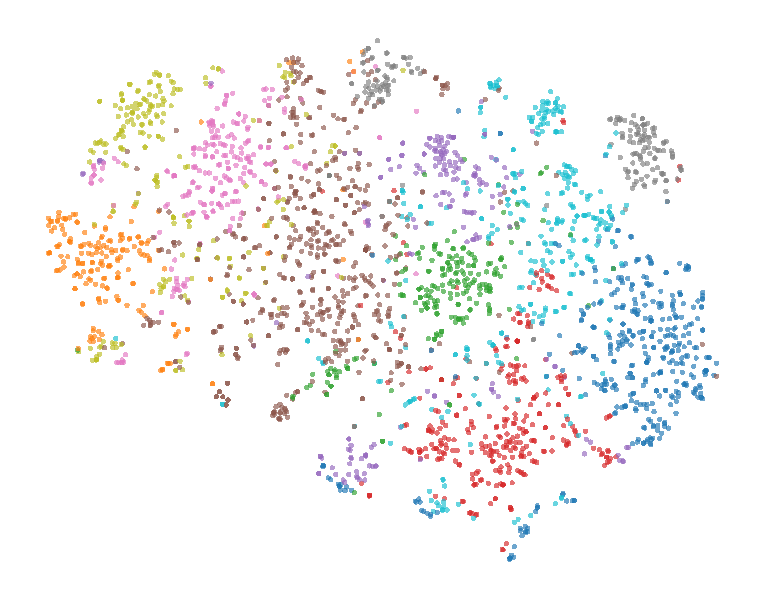
\includegraphics[width=\columnwidth]{votr_tsne.pdf}
\caption{2D projection (PCA + t-SNE) of all 2,806 tool embeddings coloured by
$k$-means cluster ($k=10$). The dense central mixing zone motivates the hybrid
BM25+SPLADE-lite stages and field-aware re-ranking.}
\label{fig:tsne}
\end{figure}

\subsection{Ablation Study}

\begin{table}[t]
\centering
\scriptsize
\caption{Component ablation on multi\_hop.large (500 hop-level decisions, OpenAI
backbone, ablation evaluation run). Significance: exact McNemar's test ($n=500$
paired decisions) vs.\ full\_stack. $^{***}p<0.001$, $^{**}p<0.01$, ns = not
significant. The bm25\_only marker reflects a statistically significant
\emph{difference} (not inferiority): BM25-only achieves higher lexical accuracy
but degrades on paraphrased intents where semantic matching is required.
Dense-only and dense+BM25 rows serve as explicit baselines for the hybrid
contribution. Session memory has no measurable effect on this suite as it does not
yet modify retrieval ranking (Section~\ref{sec:robustness}).}
\label{tab:ablation}
\begin{tabular}{@{}lcccccc@{}}
\toprule
Profile & Top-1 & Top-5 & Hd@$k$ & Avg $k$ & Chain@1 & Sig. \\
\midrule
\textit{Baselines:} & & & & & & \\
dense\_only (MCP-Zero-style) & 0.938 & 0.952 & 0.952 & 4.984 & 0.790 & $^{**}$ \\
bm25\_only (lexical)         & 0.990 & 0.998 & 0.998 & 4.996 & 0.960 & $^{***}$ \\
\textit{Hybrid variants:} & & & & & & \\
dense\_bm25  & 0.942 & 0.986 & 0.980 & 3.576 & 0.810 & $^{**}$ \\
full\_stack  & 0.964 & 0.990 & 0.982 & 2.906 & 0.870 & -- \\
no\_handoff  & 0.964 & 0.990 & 0.992 & 8.000 & 0.870 & ns \\
no\_session  & 0.964 & 0.990 & 0.982 & 2.906 & 0.870 & ns \\
\bottomrule
\end{tabular}
\end{table}

The ablation run uses a separate evaluation configuration from the primary
evaluation; the full\_stack row reports 96.4\% Top-1 vs.\ 96.8\% in the primary
evaluation due to minor configuration differences (e.g., random seed, server
ordering).
The 2.2pp gap between dense+BM25 and full\_stack is attributable to SPLADE-lite's
bigram compound-term matching and field-aware re-ranking's disambiguation of
near-identical descriptions.
Disabling the handoff policy increases average handoff-$k$ to 8.0 without improving
Top-1, confirming that the policy controls context budget without degrading
retrieval ranking.
The BM25-only result (99.0\% Top-1) is a notable finding: lexical matching
outperforms dense retrieval on single-tool routing, but degrades on paraphrased
multi-hop intents where semantic understanding is required.

\subsection{Efficiency and Adaptive-$k$ Policy}

\begin{table}[t]
\centering
\small
\caption{Token cost comparison (tiktoken cl100k\_base).}
\label{tab:tokens}
\begin{tabular}{@{}lccc@{}}
\toprule
Format & Mean/tool & At $k=3$ & Reduction \\
\midrule
\mcpzero (published Fig.~2)           & $\sim$143 & $\sim$429 & -- \\
\mcpzero-style (indexed, $n=2{,}806$) & 93.5      & 281       & -- \\
Compressed (\votr)                    & 26.2      & 79        & 72\% \\
\votr end-to-end mean (500 queries)   & --        & 230.3     & 99.91\% vs full-cat. \\
\bottomrule
\end{tabular}
\end{table}

\begin{table}[t]
\centering
\small
\caption{Fixed-$k$ vs.\ adaptive policy on single\_tool.large ($n=500$, primary
evaluation). The adaptive policy matches fixed $k=3$ accuracy at slightly lower
average token cost, while resolving 30\% of queries with a single injected tool.}
\label{tab:fixedk}
\begin{tabular}{@{}lccc@{}}
\toprule
Policy & Avg $k$ & Handoff@$k$ & Tokens/query \\
\midrule
Fixed $k=1$       & 1.0   & 0.968 & 26 \\
Fixed $k=3$       & 3.0   & 0.980 & 79 \\
Fixed $k=5$       & 5.0   & 0.990 & 131 \\
Adaptive (\votr)  & 3.38  & 0.984 & 88 \\
\bottomrule
\end{tabular}
\end{table}

Table~\ref{tab:fixedk} quantifies the adaptive policy's value: it achieves 98.4\%
Handoff@$k$---higher than fixed $k=3$ (98.0\%)---while resolving 30\% of queries
with a single injected tool (26 tokens) and expanding to $k=5$ for ambiguous
queries.
The improvement over fixed $k=3$ is modest (0.4pp) but the policy provides genuine
uncertainty discrimination: it correctly identifies which queries need more
candidates.

Median end-to-end routing latency is 312\,ms (P95: 393\,ms), dominated by the
OpenAI embedding API round-trip; local retrieval and re-ranking add under 20\,ms.

\begin{table}[t]
\centering
\caption{Confidence tier accuracy on single\_tool.large ($n=500$, primary
evaluation). The policy correctly identifies harder queries: 56\% of strict Top-1
misses occur in the low-confidence tier.}
\label{tab:confidence}
\begin{tabular}{@{}lcccc@{}}
\toprule
Tier    & Count (\%)    & Top-1 & Handoff@$k$ & Avg $k$ \\
\midrule
High    & 150\,(30.0)   & 0.967 & 0.967       & 1.0 \\
Medium  & 105\,(21.0)   & 1.000 & 1.000       & 3.0 \\
Low     & 245\,(49.0)   & 0.947 & 0.984       & 5.0 \\
Overall & 500\,(100.0)  & 0.968 & 0.984       & 3.4 \\
\bottomrule
\end{tabular}
\end{table}

\begin{figure}[t]
\centering
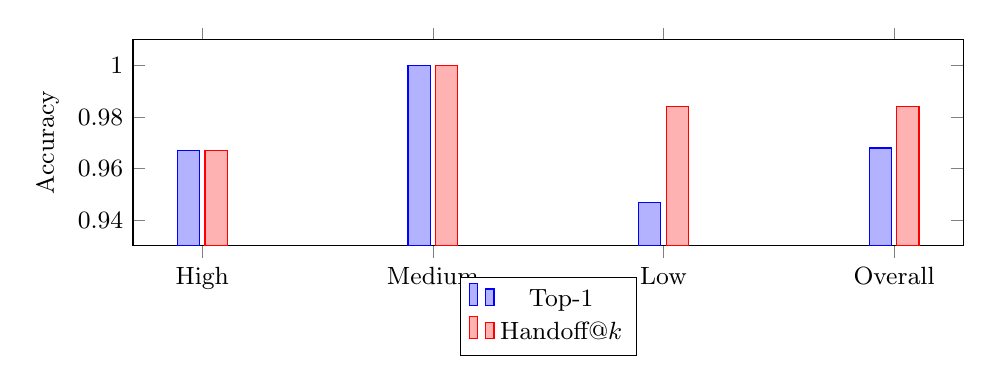
\begin{tikzpicture}
\begin{axis}[
    ybar, bar width=8pt, ymin=0.93, ymax=1.01, xtick=data,
    symbolic x coords={High,Medium,Low,Overall},
    legend style={at={(0.5,-0.15)}, anchor=north, font=\small},
    ylabel={Accuracy}, width=\columnwidth, height=4.2cm,
    tick label style={font=\small}, label style={font=\small}
]
\addplot coordinates {(High,0.967)(Medium,1.000)(Low,0.947)(Overall,0.968)};
\addplot coordinates {(High,0.967)(Medium,1.000)(Low,0.984)(Overall,0.984)};
\legend{Top-1, Handoff@$k$}
\end{axis}
\end{tikzpicture}
\caption{Accuracy by confidence tier (single\_tool.large, primary evaluation).
Low-confidence routing recovers 3.7pp through the expanded candidate set,
validating the adaptive-$k$ design.}
\label{fig:confidence}
\end{figure}

\subsection{Embedding Backbone Comparison}
\label{sec:backbone}

\begin{table}[t]
\centering
\small
\caption{Embedding backbone comparison on multi\_hop.large ($n=500$ hops, ablation
run). BGE provides the best accuracy-latency-cost tradeoff for cost-sensitive
deployments. Gemini Embedding 2 Preview's high observed P50 (3,607\,ms) reflects
provider-side rate limiting and quota pacing in our evaluation run rather than
fundamental model latency; results should be interpreted accordingly.}
\label{tab:backbone}
\begin{tabular}{@{}lcccc@{}}
\toprule
Backbone & Top-1 & Chain@1 & P50\,ms & Cost \\
\midrule
OpenAI 3-large  & 0.964 & 0.870 & 312  & API \\
Gemini Embed 2  & 0.968 & 0.890 & 3607 & API \\
BGE large-en    & 0.962 & 0.860 & 141  & local \\
Qwen3-8B        & 0.948 & 0.810 & 146  & local \\
Gemma-300M      & 0.878 & 0.620 & 151  & local \\
\bottomrule
\end{tabular}
\end{table}

BGE achieves 96.2\% Top-1 at 141\,ms P50 with no per-query API cost, making it
the recommended backbone for latency-sensitive or cost-constrained deployments.
Gemma-300M's lower accuracy (87.8\%) reflects the limits of a 300M-parameter model
on identifier-heavy MCP vocabulary.

\subsection{External Validation and Adversarial Analysis}
\label{sec:external}

\begin{table}[t]
\centering
\scriptsize
\caption{LiveMCPBench evaluation~\cite{livemcpbench2025}. ``Native dual-field''
uses \votr's structured \texttt{server\_intent} + \texttt{tool\_intent} API;
step-query rows collapse both fields to a single string.
$^\dagger$nDCG@5 from~\cite{tool_to_agent_2025}; step-query protocol only.}
\label{tab:livemcp}
\begin{tabular}{@{}lcccc@{}}
\toprule
Protocol & $n$ & R@1 & R@5 & nDCG@5 \\
\midrule
Step-query/server (Full95 reconstructed)       & 268 & 0.524 & 0.660 & 0.599 \\
Paper-faithful tool-to-agent~\cite{tool_to_agent_2025} & 82 & 0.707 & 0.878 & 0.799 \\
Tool-to-Agent Retrieval~\cite{tool_to_agent_2025}      & --  & 0.610 & 0.830 & 0.460$^\dagger$ \\
\votr native dual-field protocol               & 268 & 0.877 & 0.927 & 0.909 \\
\bottomrule
\end{tabular}
\end{table}

Under the native dual-field protocol, \votr achieves 87.7\% Recall@1 on
LiveMCPBench.
For context, Tool-to-Agent Retrieval~\cite{tool_to_agent_2025} reports 61.0\%
Recall@1 under the comparable step-query protocol---a protocol that, when applied
to \votr, yields 52.4\%, indicating that the 26.3pp gap is attributable primarily
to input format requirements rather than retrieval quality differences.
The 35.3pp gap between step-query and native dual-field reflects an interface
contract difference: \votr's \texttt{/route} endpoint accepts two structured fields
because server routing and tool selection are distinct sub-problems.
Tool-to-Agent Retrieval reports higher step-query recall through bipartite graph
joint indexing of tools and agents---a structural representation \votr does not
currently model, and a promising extension.
Notably, \votr achieves higher nDCG@5 (0.599 vs.\ 0.460$^\dagger$) under the
comparable protocol, indicating competitive ranking quality once relevant candidates
are retrieved.

The dynamic registration experiment confirms zero-impact hot registration:
pre-registration Miss@5 rate 100\%, post-registration Hit@1 100\%, with original
control queries preserved at 100\% accuracy.

Table~\ref{tab:adv} reports adversarial evaluation results.
The 16-query regression suite achieves 100\% abstention pass rate.
Under the pure adversarial 50-hop variant---deliberately ambiguous server names and
misleading surface cues---chain success falls to 0\% (hop-level Top-1: 0\%), while
the adversarial valid variant (paraphrased but grounded intents) achieves 90\%
hop-level Top-$k$ despite 0\% chain success at $k=1$.
The failure mode is coordinated metadata manipulation: when an attacker controls
server descriptions to embed misleading surface terms, both BM25's lexical matching
and dense retrieval's semantic similarity can be exploited simultaneously.
This attack surface is relevant primarily in open-registry deployments;
enterprise deployments with curated catalogues are not exposed to this failure mode.
A cross-encoder re-ranking stage~\cite{nogueira2019bert} is the primary planned
mitigation.

\begin{table}[t]
\centering
\scriptsize
\caption{Adversarial and negative control results.}
\label{tab:adv}
\begin{tabular}{@{}lccccc@{}}
\toprule
Suite & Cases & Hops & Hop@1 & Hop@$k$ & Pass Rate \\
\midrule
Regression (unsupported)      & 8 & --  & --    & --    & 1.000 \\
Regression (adversarial)      & 8 & --  & --    & --    & 1.000 \\
50-hop adversarial (valid)    & 1 & 50  & 0.580 & 0.900 & -- \\
50-hop adversarial (pure)     & 1 & 50  & 0.000 & 0.000 & -- \\
\bottomrule
\end{tabular}
\end{table}

\subsection{System Properties}

\begin{table}[t]
\centering
\small
\caption{System properties at 309-server / 2,806-tool scale.}
\label{tab:system}
\begin{tabular}{@{}lll@{}}
\toprule
Property & \mcpzero & \votr \\
\midrule
Index memory (embeddings) & $\sim$326\,MB (JSON) & $\sim$40\,MB (.npy shards) \\
Routing P50 latency    & not reported         & 312\,ms (OpenAI) / 141\,ms (BGE) \\
Hot registration       & not supported        & atomic swap, zero downtime \\
Concurrent safety      & not reported         & GIL-atomic index swap \\
Abstention mechanism   & none                 & two-stage support guard \\
\bottomrule
\end{tabular}
\end{table}

Table~\ref{tab:system} summarises system-level properties.
The \texttt{.npy} shard format stores dense embedding arrays in approximately 40\,MB
(measured: 3.6\,MB server description + 3.6\,MB server summary + 32.9\,MB tool
embeddings), compared to \mcpzero's 326\,MB JSON.
Hot registration is atomic under CPython's GIL: the index swap is a single
reference assignment, so in-flight requests complete against the pre-swap index
while subsequent requests immediately use the updated index.

%% ============================================================
\section{Discussion and Limitations}
%% ============================================================

\subsection{Hybrid Retrieval Analysis}
BM25-only achieves 99.0\% Top-1 on multi-hop routing but degrades on paraphrased
intents, which is why full\_stack is the deployment choice despite BM25-only's
lexical advantage.
A query such as ``manage user notification preferences'' requires semantic
understanding to match \texttt{update\_notification\_settings}, sharing no lexical
overlap.
Dense retrieval handles this class; hybrid ensures neither failure mode dominates.

\subsection{Error Analysis}
Of 16 Top-1 misses on single\_tool.large (primary evaluation, OpenAI backbone):
13 are near-misses (correct tool appears in top-3 or top-5, typically due to
cross-server capability overlap or server-name aliasing);
3 are semantic failures where BM25 retrieves the correct tool but dense retrieval
ranks a semantically similar tool from a competing server higher.
Zero misses are hard cases where neither BM25 nor dense retrieval identifies the
correct tool in the top-5.
This breakdown confirms that the primary failure mode is cross-server overlap
rather than fundamental retrieval failure, and that the overlap-aware disambiguation
mechanism (Section~\ref{sec:robustness}) is the correct mitigation target.

\subsection{Confidence Policy}
The confidence tiers cover roughly 30\%, 21\%, and 49\% of large-suite queries,
with average handoff-$k$ of 3.4.
The policy demonstrates genuine uncertainty discrimination: 56\% of all Top-1 misses
arise in the low-confidence tier despite it containing only 49\% of queries.

\subsection{Limitations}
\begin{itemize}
\item \textbf{Closed-catalogue evaluation:} Functional-correctness benchmarks
  measure routing accuracy within the indexed catalogue. Generalisation to novel
  server descriptions is validated only through LiveMCPBench and dynamic
  registration.
\item \textbf{Embedding API dependency:} OpenAI API calls account for
  $\sim$200--280\,ms of total latency. BGE reduces P50 by 55\% at a 0.2pp Top-1
  cost.
\item \textbf{Adversarial metadata vulnerability:} Coordinated manipulation of
  server descriptions can bypass retrieval (Section~\ref{sec:external}).
  Cross-encoder re-ranking~\cite{nogueira2019bert} is the primary planned
  mitigation.
\item \textbf{No online feedback:} Session memory records prior tool injections but
  does not yet bias retrieval.
\item \textbf{Interface sensitivity:} Step-query LiveMCPBench recall (52.4\%)
  vs.\ native protocol (87.7\%) reflects input format requirements.
\item \textbf{No direct baseline comparison:} RAG-MCP and Dynamic ReAct lack public
  implementations compatible with our benchmark protocol.
\item \textbf{No human evaluation:} Automatic retrieval metrics may not fully
  capture downstream routing quality or schema usability from a developer
  perspective.
\end{itemize}

%% ============================================================
\section{Conclusion}
%% ============================================================

\votr is a production-deployable tool retrieval service for MCP-based LLM agent
systems.
On a 500-query benchmark spanning 309 servers and 2,806 tools, \votr achieves
96.8\% Top-1 accuracy [95\% CI: 95.0, 98.2] at sub-350ms median latency with an
average context injection of 230 tokens---a 99.91\% reduction relative to
full-catalogue injection.
Multi-hop chains over 50 unique servers achieve 100\% chain success; 5-step
compound chains achieve 87\% at $k=1$.

The ablation study demonstrates that hybrid retrieval combining dense embeddings,
BM25, and SPLADE-lite via weighted RRF consistently outperforms any single retrieval
signal.
The calibrated score-gap policy achieves higher Handoff@$k$ than fixed $k=3$ at
comparable average token cost, resolving 30\% of queries with a single injected
tool.
BGE provides a viable local-embedding alternative at 141\,ms P50 and 96.2\% Top-1.

Graph-aware joint tool-agent retrieval and cross-encoder re-ranking represent the
primary planned extensions to address the interface sensitivity and adversarial
robustness limitations identified.

\begin{acks}
Acknowledgements omitted for blind review.
\end{acks}

\bibliographystyle{ACM-Reference-Format}
\bibliography{votr_cikm2026}

\end{document}
